% Options for packages loaded elsewhere
\PassOptionsToPackage{unicode}{hyperref}
\PassOptionsToPackage{hyphens}{url}
%
\documentclass[
]{article}
\usepackage{amsmath,amssymb}
\usepackage{iftex}
\ifPDFTeX
  \usepackage[T1]{fontenc}
  \usepackage[utf8]{inputenc}
  \usepackage{textcomp} % provide euro and other symbols
\else % if luatex or xetex
  \usepackage{unicode-math} % this also loads fontspec
  \defaultfontfeatures{Scale=MatchLowercase}
  \defaultfontfeatures[\rmfamily]{Ligatures=TeX,Scale=1}
\fi
\usepackage{lmodern}
\ifPDFTeX\else
  % xetex/luatex font selection
\fi
% Use upquote if available, for straight quotes in verbatim environments
\IfFileExists{upquote.sty}{\usepackage{upquote}}{}
\IfFileExists{microtype.sty}{% use microtype if available
  \usepackage[]{microtype}
  \UseMicrotypeSet[protrusion]{basicmath} % disable protrusion for tt fonts
}{}
\makeatletter
\@ifundefined{KOMAClassName}{% if non-KOMA class
  \IfFileExists{parskip.sty}{%
    \usepackage{parskip}
  }{% else
    \setlength{\parindent}{0pt}
    \setlength{\parskip}{6pt plus 2pt minus 1pt}}
}{% if KOMA class
  \KOMAoptions{parskip=half}}
\makeatother
\usepackage{xcolor}
\usepackage[margin=1in]{geometry}
\usepackage{color}
\usepackage{fancyvrb}
\newcommand{\VerbBar}{|}
\newcommand{\VERB}{\Verb[commandchars=\\\{\}]}
\DefineVerbatimEnvironment{Highlighting}{Verbatim}{commandchars=\\\{\}}
% Add ',fontsize=\small' for more characters per line
\usepackage{framed}
\definecolor{shadecolor}{RGB}{248,248,248}
\newenvironment{Shaded}{\begin{snugshade}}{\end{snugshade}}
\newcommand{\AlertTok}[1]{\textcolor[rgb]{0.94,0.16,0.16}{#1}}
\newcommand{\AnnotationTok}[1]{\textcolor[rgb]{0.56,0.35,0.01}{\textbf{\textit{#1}}}}
\newcommand{\AttributeTok}[1]{\textcolor[rgb]{0.13,0.29,0.53}{#1}}
\newcommand{\BaseNTok}[1]{\textcolor[rgb]{0.00,0.00,0.81}{#1}}
\newcommand{\BuiltInTok}[1]{#1}
\newcommand{\CharTok}[1]{\textcolor[rgb]{0.31,0.60,0.02}{#1}}
\newcommand{\CommentTok}[1]{\textcolor[rgb]{0.56,0.35,0.01}{\textit{#1}}}
\newcommand{\CommentVarTok}[1]{\textcolor[rgb]{0.56,0.35,0.01}{\textbf{\textit{#1}}}}
\newcommand{\ConstantTok}[1]{\textcolor[rgb]{0.56,0.35,0.01}{#1}}
\newcommand{\ControlFlowTok}[1]{\textcolor[rgb]{0.13,0.29,0.53}{\textbf{#1}}}
\newcommand{\DataTypeTok}[1]{\textcolor[rgb]{0.13,0.29,0.53}{#1}}
\newcommand{\DecValTok}[1]{\textcolor[rgb]{0.00,0.00,0.81}{#1}}
\newcommand{\DocumentationTok}[1]{\textcolor[rgb]{0.56,0.35,0.01}{\textbf{\textit{#1}}}}
\newcommand{\ErrorTok}[1]{\textcolor[rgb]{0.64,0.00,0.00}{\textbf{#1}}}
\newcommand{\ExtensionTok}[1]{#1}
\newcommand{\FloatTok}[1]{\textcolor[rgb]{0.00,0.00,0.81}{#1}}
\newcommand{\FunctionTok}[1]{\textcolor[rgb]{0.13,0.29,0.53}{\textbf{#1}}}
\newcommand{\ImportTok}[1]{#1}
\newcommand{\InformationTok}[1]{\textcolor[rgb]{0.56,0.35,0.01}{\textbf{\textit{#1}}}}
\newcommand{\KeywordTok}[1]{\textcolor[rgb]{0.13,0.29,0.53}{\textbf{#1}}}
\newcommand{\NormalTok}[1]{#1}
\newcommand{\OperatorTok}[1]{\textcolor[rgb]{0.81,0.36,0.00}{\textbf{#1}}}
\newcommand{\OtherTok}[1]{\textcolor[rgb]{0.56,0.35,0.01}{#1}}
\newcommand{\PreprocessorTok}[1]{\textcolor[rgb]{0.56,0.35,0.01}{\textit{#1}}}
\newcommand{\RegionMarkerTok}[1]{#1}
\newcommand{\SpecialCharTok}[1]{\textcolor[rgb]{0.81,0.36,0.00}{\textbf{#1}}}
\newcommand{\SpecialStringTok}[1]{\textcolor[rgb]{0.31,0.60,0.02}{#1}}
\newcommand{\StringTok}[1]{\textcolor[rgb]{0.31,0.60,0.02}{#1}}
\newcommand{\VariableTok}[1]{\textcolor[rgb]{0.00,0.00,0.00}{#1}}
\newcommand{\VerbatimStringTok}[1]{\textcolor[rgb]{0.31,0.60,0.02}{#1}}
\newcommand{\WarningTok}[1]{\textcolor[rgb]{0.56,0.35,0.01}{\textbf{\textit{#1}}}}
\usepackage{longtable,booktabs,array}
\usepackage{calc} % for calculating minipage widths
% Correct order of tables after \paragraph or \subparagraph
\usepackage{etoolbox}
\makeatletter
\patchcmd\longtable{\par}{\if@noskipsec\mbox{}\fi\par}{}{}
\makeatother
% Allow footnotes in longtable head/foot
\IfFileExists{footnotehyper.sty}{\usepackage{footnotehyper}}{\usepackage{footnote}}
\makesavenoteenv{longtable}
\usepackage{graphicx}
\makeatletter
\def\maxwidth{\ifdim\Gin@nat@width>\linewidth\linewidth\else\Gin@nat@width\fi}
\def\maxheight{\ifdim\Gin@nat@height>\textheight\textheight\else\Gin@nat@height\fi}
\makeatother
% Scale images if necessary, so that they will not overflow the page
% margins by default, and it is still possible to overwrite the defaults
% using explicit options in \includegraphics[width, height, ...]{}
\setkeys{Gin}{width=\maxwidth,height=\maxheight,keepaspectratio}
% Set default figure placement to htbp
\makeatletter
\def\fps@figure{htbp}
\makeatother
\setlength{\emergencystretch}{3em} % prevent overfull lines
\providecommand{\tightlist}{%
  \setlength{\itemsep}{0pt}\setlength{\parskip}{0pt}}
\setcounter{secnumdepth}{-\maxdimen} % remove section numbering
\usepackage{booktabs}
\usepackage{longtable}
\usepackage{array}
\usepackage{multirow}
\usepackage{wrapfig}
\usepackage{float}
\usepackage{colortbl}
\usepackage{pdflscape}
\usepackage{tabu}
\usepackage{threeparttable}
\usepackage{threeparttablex}
\usepackage[normalem]{ulem}
\usepackage{makecell}
\usepackage{xcolor}
\ifLuaTeX
  \usepackage{selnolig}  % disable illegal ligatures
\fi
\IfFileExists{bookmark.sty}{\usepackage{bookmark}}{\usepackage{hyperref}}
\IfFileExists{xurl.sty}{\usepackage{xurl}}{} % add URL line breaks if available
\urlstyle{same}
\hypersetup{
  pdftitle={Ejemplo de R Markdown: El voto autonómico en la comarca de la Safor (VALENCIA)},
  pdfauthor={Tomàs Ferrandis Moscardó},
  hidelinks,
  pdfcreator={LaTeX via pandoc}}

\title{Ejemplo de R Markdown: \emph{El voto autonómico en la comarca de
la Safor (VALENCIA)}}
\author{Tomàs Ferrandis Moscardó}
\date{2024-01-26}

\begin{document}
\maketitle

{
\setcounter{tocdepth}{2}
\tableofcontents
}
\hypertarget{introducciuxf3n}{%
\section{INTRODUCCIÓN}\label{introducciuxf3n}}

A continuación veremos un sencillo ejemplo de uso de \textbf{R-Markdown}
en el que, a partir de un fichero de tipo \emph{csv} ( SAFOR.csv )
crearemos y manipularemos objetos \emph{data.frame}. Obtendremos algunas
medidas de \emph{tendencia central y dispersión} que representaremos en
tablas y gráficos.

Después guardaremos los datos del data\_frame de resultados en ficheros
de diversos tipos: \emph{csv, xlsx, dta, RData, sav, rds)}

\hypertarget{inclusiuxf3n-de-los-paquetes-y-sus-libreruxedas-que-vamos-a-necesitar}{%
\subsection{Inclusión de los paquetes ( y sus librerías) que vamos a
necesitar}\label{inclusiuxf3n-de-los-paquetes-y-sus-libreruxedas-que-vamos-a-necesitar}}

Las librerías se cargan solo si previamente se ha instalado el paquete
que las contiene. En nuestros \emph{chuncks} ( pedazos de código R),
comprobaremos si están disponibles. Solo en caso contrario instalaremos
su paquete correspondiente. Se intenta cargar una librería mediante
\emph{require()} . Si da error, require devuelve un valor FALSE
(!require()), entonces se ejecuta la instalación del paquete (que carga
también la librería).

\begin{Shaded}
\begin{Highlighting}[]
\CommentTok{\# Requisitos previes. Paquetes y librerías}
\ControlFlowTok{if}\NormalTok{ (}\SpecialCharTok{!}\FunctionTok{require}\NormalTok{(}\StringTok{"dplyr"}\NormalTok{)) \{}\FunctionTok{install.packages}\NormalTok{(}\StringTok{"dplyr"}\NormalTok{)\}}
\ControlFlowTok{if}\NormalTok{ (}\SpecialCharTok{!}\FunctionTok{require}\NormalTok{(}\StringTok{"stringr"}\NormalTok{)) \{}\FunctionTok{install.packages}\NormalTok{(}\StringTok{"stringr"}\NormalTok{)\}}
\ControlFlowTok{if}\NormalTok{ (}\SpecialCharTok{!}\FunctionTok{require}\NormalTok{(}\StringTok{"curl"}\NormalTok{)) \{}\FunctionTok{install.packages}\NormalTok{(}\StringTok{"curl"}\NormalTok{)\}}
\ControlFlowTok{if}\NormalTok{ (}\SpecialCharTok{!}\FunctionTok{require}\NormalTok{(}\StringTok{"rsconnect"}\NormalTok{))\{}\FunctionTok{install.packages}\NormalTok{(}\StringTok{"rsconnect"}\NormalTok{)\}}
\ControlFlowTok{if}\NormalTok{ (}\SpecialCharTok{!}\FunctionTok{require}\NormalTok{(}\StringTok{"kableExtra"}\NormalTok{))\{}\FunctionTok{install.packages}\NormalTok{(}\StringTok{"kableExtra"}\NormalTok{)\}}
\ControlFlowTok{if}\NormalTok{ (}\SpecialCharTok{!}\FunctionTok{require}\NormalTok{(}\StringTok{"tidyverse"}\NormalTok{))\{}\FunctionTok{install.packages}\NormalTok{(}\StringTok{"tidyverse"}\NormalTok{)\}}
\FunctionTok{library}\NormalTok{(data.table)}
\FunctionTok{library}\NormalTok{(knitr)}
\FunctionTok{library}\NormalTok{(stringr)}
\FunctionTok{library}\NormalTok{(dplyr)}
\FunctionTok{library}\NormalTok{(ggplot2)}
\end{Highlighting}
\end{Shaded}

\hypertarget{obtenciuxf3n-y-tratamiento-de-los-datos}{%
\section{OBTENCIÓN Y TRATAMIENTO DE LOS
DATOS}\label{obtenciuxf3n-y-tratamiento-de-los-datos}}

\hypertarget{resultados-de-todas-las-elecciones-y-convocatorias-a-nivel-de-agregaciuxf3n-comarcal.-caso-de-la-safor.}{%
\subsection{Resultados de todas las elecciones y convocatorias a nivel
de agregación comarcal. Caso de La
Safor.}\label{resultados-de-todas-las-elecciones-y-convocatorias-a-nivel-de-agregaciuxf3n-comarcal.-caso-de-la-safor.}}

A partir de la base de datos de ARGOS descargamos el resumen de
resultados electorales en las distintas convocatorias y procesos
electorales en un fichero \emph{CSV}.

\begin{Shaded}
\begin{Highlighting}[]
\NormalTok{  df1}\OtherTok{\textless{}{-}}\FunctionTok{read.csv}\NormalTok{(}\StringTok{"CSV/SAFOR.csv"}\NormalTok{,}\AttributeTok{header=}\ConstantTok{TRUE}\NormalTok{, }\AttributeTok{sep=}\StringTok{","}\NormalTok{,}\AttributeTok{quote=}\StringTok{"}\SpecialCharTok{\textbackslash{}"}\StringTok{\textquotesingle{}"}\NormalTok{, }\AttributeTok{dec=}\StringTok{","}\NormalTok{,}\AttributeTok{fill=}\ConstantTok{TRUE}\NormalTok{,}
                \AttributeTok{comment.char =} \StringTok{""}\NormalTok{)}
  \CommentTok{\# View(df1) \# Para ver en consola}
\end{Highlighting}
\end{Shaded}

Veamos como ejemplo las primeras líneas\ldots{}

\begin{Shaded}
\begin{Highlighting}[]
\FunctionTok{head}\NormalTok{(df1)}
\end{Highlighting}
\end{Shaded}

\begin{verbatim}
##   Elecció   Cens A.Cand.    PP  PSPV COMPROMÍS   VOX PODEMOS   Cs EUPV RESTA
## 1  G-2023 124383   90477 29545 31386     15855 12462      NA   NA   NA  1229
## 2  A-2023 124367   86496 28245 25559     19953  8282    2234  591   NA  1859
## 3  L-2023 127096   88398 27174 28953     15703  3126     120  364 1143 11795
## 4  G-2019 121791   86427 19634 23322     10644 14008   11334 5559   NA  1926
## 5  E-2019 123535   84970 19128 25797     15919  4818    6621 8761   NA  3926
## 6  L-2019 124552   86268 23328 26289     19803  1910    1155 4541 1197  8044
\end{verbatim}

\hypertarget{filtramos-por-elecciones-autonuxf3micas.}{%
\subsection{Filtramos por elecciones
autonómicas.}\label{filtramos-por-elecciones-autonuxf3micas.}}

Asumimos como \textbf{universo o población} el conjunto de todas las
todas elecciones autonómicas.

\hypertarget{filtraremos-por-el-campo-correspondiente}{%
\subsection{Filtraremos por el campo
correspondiente}\label{filtraremos-por-el-campo-correspondiente}}

\begin{Shaded}
\begin{Highlighting}[]
\NormalTok{df\_autonomicas}\OtherTok{\textless{}{-}}\NormalTok{df1 }\SpecialCharTok{\%\textgreater{}\%} \FunctionTok{filter}\NormalTok{(}\FunctionTok{str\_detect}\NormalTok{(df1}\SpecialCharTok{$}\NormalTok{Elecció,}\StringTok{"A{-}"}\NormalTok{))}
\end{Highlighting}
\end{Shaded}

\hypertarget{vemos-las-primeras-lineas-de-ejemplo}{%
\subsection{Vemos las primeras lineas de
ejemplo}\label{vemos-las-primeras-lineas-de-ejemplo}}

\begin{Shaded}
\begin{Highlighting}[]
\FunctionTok{head}\NormalTok{(df\_autonomicas)}
\end{Highlighting}
\end{Shaded}

\begin{verbatim}
##   Elecció   Cens A.Cand.    PP  PSPV COMPROMÍS  VOX PODEMOS    Cs EUPV RESTA
## 1  A-2023 124367   86496 28245 25559     19953 8282    2234   591   NA  1859
## 2  A-2019 121181   89534 17325 19867     23504 7666    5917 12394   NA  2861
## 3  A-2015 121362   90086 26377 18226     24789  207    6845  7668 3129  2845
## 4  A-2011 120877   92475 47413 25159     12366   NA      NA    NA 3323  4214
## 5  A-2007 119109   90705 46558 29321     11050   NA      NA    NA   NA  3776
## 6  A-2003 116160   90337 41220 31192     10891   NA      NA    NA 3145  3889
\end{verbatim}

\hypertarget{tratamiento-de-los-na}{%
\subsection{Tratamiento de los NA}\label{tratamiento-de-los-na}}

En nuestro caso los NA se deben a la ausencia de resultados por no
haberse presentado la fuerza política en una convocatoria o por haberse
integrado en una coalición electoral. Entendemos que el valor que debe
sustituir NA para poder realizar cálculos estadísticos de forma correcta
y sin errores de computación es el 0. Podríamos recorrer solo las
columnas de partidos pero lo simplificamos y aplicamos la sustitución NA
-\textgreater{} 0 en todo el data frame.

\begin{Shaded}
\begin{Highlighting}[]
\NormalTok{df\_autonomicas[}\FunctionTok{is.na}\NormalTok{(df\_autonomicas)]}\OtherTok{\textless{}{-}}\DecValTok{0}
\end{Highlighting}
\end{Shaded}

Mostramos los datos en formato de tabla de RMarkdown

\begin{Shaded}
\begin{Highlighting}[]
\NormalTok{knitr}\SpecialCharTok{::}\FunctionTok{kable}\NormalTok{(df\_autonomicas, }\AttributeTok{caption =} \StringTok{"ELECCIONES AUTONÓMICAS EN LA SAFOR"}\NormalTok{)}
\end{Highlighting}
\end{Shaded}

\begin{longtable}[]{@{}
  >{\raggedright\arraybackslash}p{(\columnwidth - 20\tabcolsep) * \real{0.1067}}
  >{\raggedleft\arraybackslash}p{(\columnwidth - 20\tabcolsep) * \real{0.0933}}
  >{\raggedleft\arraybackslash}p{(\columnwidth - 20\tabcolsep) * \real{0.1067}}
  >{\raggedleft\arraybackslash}p{(\columnwidth - 20\tabcolsep) * \real{0.0800}}
  >{\raggedleft\arraybackslash}p{(\columnwidth - 20\tabcolsep) * \real{0.0800}}
  >{\raggedleft\arraybackslash}p{(\columnwidth - 20\tabcolsep) * \real{0.1333}}
  >{\raggedleft\arraybackslash}p{(\columnwidth - 20\tabcolsep) * \real{0.0667}}
  >{\raggedleft\arraybackslash}p{(\columnwidth - 20\tabcolsep) * \real{0.1067}}
  >{\raggedleft\arraybackslash}p{(\columnwidth - 20\tabcolsep) * \real{0.0800}}
  >{\raggedleft\arraybackslash}p{(\columnwidth - 20\tabcolsep) * \real{0.0667}}
  >{\raggedleft\arraybackslash}p{(\columnwidth - 20\tabcolsep) * \real{0.0800}}@{}}
\caption{ELECCIONES AUTONÓMICAS EN LA SAFOR}\tabularnewline
\toprule\noalign{}
\begin{minipage}[b]{\linewidth}\raggedright
Elecció
\end{minipage} & \begin{minipage}[b]{\linewidth}\raggedleft
Cens
\end{minipage} & \begin{minipage}[b]{\linewidth}\raggedleft
A.Cand.
\end{minipage} & \begin{minipage}[b]{\linewidth}\raggedleft
PP
\end{minipage} & \begin{minipage}[b]{\linewidth}\raggedleft
PSPV
\end{minipage} & \begin{minipage}[b]{\linewidth}\raggedleft
COMPROMÍS
\end{minipage} & \begin{minipage}[b]{\linewidth}\raggedleft
VOX
\end{minipage} & \begin{minipage}[b]{\linewidth}\raggedleft
PODEMOS
\end{minipage} & \begin{minipage}[b]{\linewidth}\raggedleft
Cs
\end{minipage} & \begin{minipage}[b]{\linewidth}\raggedleft
EUPV
\end{minipage} & \begin{minipage}[b]{\linewidth}\raggedleft
RESTA
\end{minipage} \\
\midrule\noalign{}
\endfirsthead
\toprule\noalign{}
\begin{minipage}[b]{\linewidth}\raggedright
Elecció
\end{minipage} & \begin{minipage}[b]{\linewidth}\raggedleft
Cens
\end{minipage} & \begin{minipage}[b]{\linewidth}\raggedleft
A.Cand.
\end{minipage} & \begin{minipage}[b]{\linewidth}\raggedleft
PP
\end{minipage} & \begin{minipage}[b]{\linewidth}\raggedleft
PSPV
\end{minipage} & \begin{minipage}[b]{\linewidth}\raggedleft
COMPROMÍS
\end{minipage} & \begin{minipage}[b]{\linewidth}\raggedleft
VOX
\end{minipage} & \begin{minipage}[b]{\linewidth}\raggedleft
PODEMOS
\end{minipage} & \begin{minipage}[b]{\linewidth}\raggedleft
Cs
\end{minipage} & \begin{minipage}[b]{\linewidth}\raggedleft
EUPV
\end{minipage} & \begin{minipage}[b]{\linewidth}\raggedleft
RESTA
\end{minipage} \\
\midrule\noalign{}
\endhead
\bottomrule\noalign{}
\endlastfoot
A-2023 & 124367 & 86496 & 28245 & 25559 & 19953 & 8282 & 2234 & 591 & 0
& 1859 \\
A-2019 & 121181 & 89534 & 17325 & 19867 & 23504 & 7666 & 5917 & 12394 &
0 & 2861 \\
A-2015 & 121362 & 90086 & 26377 & 18226 & 24789 & 207 & 6845 & 7668 &
3129 & 2845 \\
A-2011 & 120877 & 92475 & 47413 & 25159 & 12366 & 0 & 0 & 0 & 3323 &
4214 \\
A-2007 & 119109 & 90705 & 46558 & 29321 & 11050 & 0 & 0 & 0 & 0 &
3776 \\
A-2003 & 116160 & 90337 & 41220 & 31192 & 10891 & 0 & 0 & 0 & 3145 &
3889 \\
A-1999 & 117654 & 87007 & 40176 & 27696 & 9066 & 0 & 0 & 0 & 3782 &
6287 \\
A-1995 & 108888 & 86600 & 32374 & 29415 & 7600 & 0 & 0 & 0 & 7503 &
9708 \\
A-1991 & 102923 & 78619 & 19181 & 30884 & 7998 & 0 & 0 & 0 & 5313 &
15243 \\
A-1987 & 97022 & 75807 & 17142 & 28744 & 0 & 0 & 0 & 0 & 9042 & 20879 \\
A-1983 & 94401 & 72681 & 22015 & 30781 & 5823 & 0 & 0 & 0 & 5815 &
8247 \\
\end{longtable}

\hypertarget{creamos-un-vector-con-las-candidaturas.}{%
\subsection{Creamos un vector con las
candidaturas.}\label{creamos-un-vector-con-las-candidaturas.}}

\begin{Shaded}
\begin{Highlighting}[]
\CommentTok{\# Recogemos los nombres de columnas a partir de la 4ª}
\NormalTok{partits}\OtherTok{\textless{}{-}}\FunctionTok{names}\NormalTok{(df1[}\DecValTok{4}\SpecialCharTok{:}\FunctionTok{length}\NormalTok{(df1)])}

\CommentTok{\# Para nuestro caso podríamos anotarlo directamente}
\CommentTok{\# partits\textless{}{-}c("PP","PSPV","COMPROMÍS","VOX","PODEMOS","Cs","EUPV","RESTA")}
\end{Highlighting}
\end{Shaded}

Los visualizamos en formato de tabla de RMarkdown

\begin{Shaded}
\begin{Highlighting}[]
\NormalTok{knitr}\SpecialCharTok{::}\FunctionTok{kable}\NormalTok{(partits, }\AttributeTok{caption =} \StringTok{"CANDIDATURAS"}\NormalTok{)}
\end{Highlighting}
\end{Shaded}

\begin{longtable}[]{@{}l@{}}
\caption{CANDIDATURAS}\tabularnewline
\toprule\noalign{}
x \\
\midrule\noalign{}
\endfirsthead
\toprule\noalign{}
x \\
\midrule\noalign{}
\endhead
\bottomrule\noalign{}
\endlastfoot
PP \\
PSPV \\
COMPROMÍS \\
VOX \\
PODEMOS \\
Cs \\
EUPV \\
RESTA \\
\end{longtable}

\hypertarget{cuxe1lculo-de-valores-de-medidas-de-tendencia-central-y-dispersiuxf3n}{%
\section{CÁLCULO DE VALORES DE MEDIDAS de TENDENCIA CENTRAL y
DISPERSIÓN}\label{cuxe1lculo-de-valores-de-medidas-de-tendencia-central-y-dispersiuxf3n}}

1.- Media o promedio 2.- Máximos 3.- Míninos 4.- Rango de variación

\begin{Shaded}
\begin{Highlighting}[]
\NormalTok{mitjana}\OtherTok{\textless{}{-}}\FunctionTok{summarise\_at}\NormalTok{(df\_autonomicas,partits,mean)}
\NormalTok{maxims}\OtherTok{\textless{}{-}}\FunctionTok{summarise\_at}\NormalTok{(df\_autonomicas,partits,max)}
\NormalTok{minims}\OtherTok{\textless{}{-}}\FunctionTok{summarise\_at}\NormalTok{(df\_autonomicas,partits,}\SpecialCharTok{\textasciitilde{}}\FunctionTok{min}\NormalTok{(.[. }\SpecialCharTok{!=} \DecValTok{0}\NormalTok{])) }\CommentTok{\#Descartamos los 0}
\NormalTok{rangodevariacion}\OtherTok{\textless{}{-}}\NormalTok{maxims }\SpecialCharTok{{-}}\NormalTok{ minims}
\end{Highlighting}
\end{Shaded}

\hypertarget{creamos-un-data-frame.-cada-vector-anterior-seruxe1-una-columna}{%
\subsection{Creamos un data frame. cada vector anterior será una
columna}\label{creamos-un-data-frame.-cada-vector-anterior-seruxe1-una-columna}}

\begin{Shaded}
\begin{Highlighting}[]
\NormalTok{df\_resultats}\OtherTok{\textless{}{-}}\FunctionTok{rbind}\NormalTok{(mitjana)}
\NormalTok{df\_resultats}\OtherTok{\textless{}{-}}\FunctionTok{rbind}\NormalTok{(df\_resultats,maxims)}
\NormalTok{df\_resultats}\OtherTok{\textless{}{-}}\FunctionTok{rbind}\NormalTok{(df\_resultats,minims)}
\NormalTok{df\_resultats}\OtherTok{\textless{}{-}}\FunctionTok{rbind}\NormalTok{(df\_resultats,rangodevariacion)}
\CommentTok{\#Redondeamos los valores a enteros ( son votos) }
\NormalTok{df\_resultats}\OtherTok{\textless{}{-}}\NormalTok{df\_resultats }\SpecialCharTok{\%\textgreater{}\%} \FunctionTok{mutate\_at}\NormalTok{(partits, as.integer)}
\end{Highlighting}
\end{Shaded}

\hypertarget{auxf1adimos-al-final-del-data-frame-una-columna-con-el-nombre-del-cuxe1lculo}{%
\subsection{Añadimos al final del data frame una columna con el nombre
del
``cálculo''}\label{auxf1adimos-al-final-del-data-frame-una-columna-con-el-nombre-del-cuxe1lculo}}

\begin{Shaded}
\begin{Highlighting}[]
\NormalTok{df\_resultats}\OtherTok{\textless{}{-}}\FunctionTok{cbind}\NormalTok{(df\_resultats,ESTADÍSTICA}\OtherTok{=}\FunctionTok{c}\NormalTok{(}\StringTok{"MEDIA"}\NormalTok{,}\StringTok{"MÁXIMO"}\NormalTok{,}\StringTok{"MÍNIMO"}\NormalTok{,}\StringTok{"RANGO"}\NormalTok{))}
\end{Highlighting}
\end{Shaded}

\begin{Shaded}
\begin{Highlighting}[]
\CommentTok{\# la resituamos en la posición 1 ( estática)}
\NormalTok{df\_resultats}\OtherTok{\textless{}{-}}\NormalTok{df\_resultats }\SpecialCharTok{\%\textgreater{}\%} \FunctionTok{select}\NormalTok{(}\StringTok{"ESTADÍSTICA"}\NormalTok{,}\FunctionTok{everything}\NormalTok{())}
\end{Highlighting}
\end{Shaded}

\hypertarget{imprimimos-en-markdown-una-tabla-con-los-resultados}{%
\subsection{Imprimimos en Markdown una tabla con los
resultados}\label{imprimimos-en-markdown-una-tabla-con-los-resultados}}

\begin{Shaded}
\begin{Highlighting}[]
\NormalTok{knitr}\SpecialCharTok{::}\FunctionTok{kable}\NormalTok{(df\_resultats, }\AttributeTok{caption =} \StringTok{"ESTADÍSTICA SAFOR"}\NormalTok{)}
\end{Highlighting}
\end{Shaded}

\begin{longtable}[]{@{}
  >{\raggedright\arraybackslash}p{(\columnwidth - 16\tabcolsep) * \real{0.1875}}
  >{\raggedleft\arraybackslash}p{(\columnwidth - 16\tabcolsep) * \real{0.0938}}
  >{\raggedleft\arraybackslash}p{(\columnwidth - 16\tabcolsep) * \real{0.0938}}
  >{\raggedleft\arraybackslash}p{(\columnwidth - 16\tabcolsep) * \real{0.1562}}
  >{\raggedleft\arraybackslash}p{(\columnwidth - 16\tabcolsep) * \real{0.0781}}
  >{\raggedleft\arraybackslash}p{(\columnwidth - 16\tabcolsep) * \real{0.1250}}
  >{\raggedleft\arraybackslash}p{(\columnwidth - 16\tabcolsep) * \real{0.0938}}
  >{\raggedleft\arraybackslash}p{(\columnwidth - 16\tabcolsep) * \real{0.0781}}
  >{\raggedleft\arraybackslash}p{(\columnwidth - 16\tabcolsep) * \real{0.0938}}@{}}
\caption{ESTADÍSTICA SAFOR}\tabularnewline
\toprule\noalign{}
\begin{minipage}[b]{\linewidth}\raggedright
ESTADÍSTICA
\end{minipage} & \begin{minipage}[b]{\linewidth}\raggedleft
PP
\end{minipage} & \begin{minipage}[b]{\linewidth}\raggedleft
PSPV
\end{minipage} & \begin{minipage}[b]{\linewidth}\raggedleft
COMPROMÍS
\end{minipage} & \begin{minipage}[b]{\linewidth}\raggedleft
VOX
\end{minipage} & \begin{minipage}[b]{\linewidth}\raggedleft
PODEMOS
\end{minipage} & \begin{minipage}[b]{\linewidth}\raggedleft
Cs
\end{minipage} & \begin{minipage}[b]{\linewidth}\raggedleft
EUPV
\end{minipage} & \begin{minipage}[b]{\linewidth}\raggedleft
RESTA
\end{minipage} \\
\midrule\noalign{}
\endfirsthead
\toprule\noalign{}
\begin{minipage}[b]{\linewidth}\raggedright
ESTADÍSTICA
\end{minipage} & \begin{minipage}[b]{\linewidth}\raggedleft
PP
\end{minipage} & \begin{minipage}[b]{\linewidth}\raggedleft
PSPV
\end{minipage} & \begin{minipage}[b]{\linewidth}\raggedleft
COMPROMÍS
\end{minipage} & \begin{minipage}[b]{\linewidth}\raggedleft
VOX
\end{minipage} & \begin{minipage}[b]{\linewidth}\raggedleft
PODEMOS
\end{minipage} & \begin{minipage}[b]{\linewidth}\raggedleft
Cs
\end{minipage} & \begin{minipage}[b]{\linewidth}\raggedleft
EUPV
\end{minipage} & \begin{minipage}[b]{\linewidth}\raggedleft
RESTA
\end{minipage} \\
\midrule\noalign{}
\endhead
\bottomrule\noalign{}
\endlastfoot
MEDIA & 30729 & 26985 & 12094 & 1468 & 1363 & 1877 & 3732 & 7255 \\
MÁXIMO & 47413 & 31192 & 24789 & 8282 & 6845 & 12394 & 9042 & 20879 \\
MÍNIMO & 17142 & 18226 & 5823 & 207 & 2234 & 591 & 3129 & 1859 \\
RANGO & 30271 & 12966 & 18966 & 8075 & 4611 & 11803 & 5913 & 19020 \\
\end{longtable}

\hypertarget{gruxe1ficos}{%
\section{GRÁFICOS}\label{gruxe1ficos}}

Vemos a continuación los gráficos y tablas de daraso a nivel de
agregación de candidatura.

\begin{Shaded}
\begin{Highlighting}[]
\CommentTok{\# Recorremos las columnas del data frame correspondientes a candidaturas ( \textgreater{}2)}
\CommentTok{\# Creamos un data frame en cada iteración}
\ControlFlowTok{for}\NormalTok{ ( i }\ControlFlowTok{in} \DecValTok{2}\SpecialCharTok{:}\FunctionTok{length}\NormalTok{(df\_resultats))\{}
\NormalTok{     df\_estPartit}\OtherTok{\textless{}{-}} \FunctionTok{data.frame}\NormalTok{(}
\NormalTok{         ESTADÍSTICA}\OtherTok{=}\NormalTok{df\_resultats}\SpecialCharTok{$}\NormalTok{ESTADÍSTICA,}
         \AttributeTok{VALORS=}\NormalTok{df\_resultats[,i],}
         \AttributeTok{PARTIT=}\FunctionTok{colnames}\NormalTok{(df\_resultats[i])}
\NormalTok{     )}

\CommentTok{\# EN UN GRAFICO}
\FunctionTok{barplot}\NormalTok{(df\_estPartit}\SpecialCharTok{$}\NormalTok{VALORS, }
        \AttributeTok{main=}\FunctionTok{paste}\NormalTok{(}\StringTok{"Valores estadísticos de"}\NormalTok{,df\_estPartit}\SpecialCharTok{$}\NormalTok{PARTIT[}\DecValTok{1}\NormalTok{]),}
        \AttributeTok{names.arg=}\NormalTok{df\_estPartit}\SpecialCharTok{$}\NormalTok{ESTADÍSTICA,}
        \AttributeTok{col=}\FunctionTok{c}\NormalTok{(}\StringTok{"\#5fe10b"}\NormalTok{,}\StringTok{"red"}\NormalTok{,}\StringTok{"\#48b7f7"}\NormalTok{,}\StringTok{"\#ede12e"}\NormalTok{),}
        \AttributeTok{ylab=}\StringTok{"VOTOS"}\NormalTok{)}


\CommentTok{\# EN UNA TABLA}
\CommentTok{\#Quitamos la columna que repite el nombre ( estético), lo guardamos antes}
\NormalTok{candidatura}\OtherTok{\textless{}{-}}\NormalTok{df\_estPartit}\SpecialCharTok{$}\NormalTok{PARTIT[}\DecValTok{1}\NormalTok{]}
\NormalTok{df\_estPartit }\OtherTok{\textless{}{-}}\NormalTok{ df\_estPartit[, }\SpecialCharTok{!}\NormalTok{(}\FunctionTok{names}\NormalTok{(df\_estPartit) }\SpecialCharTok{\%in\%} \StringTok{"PARTIT"}\NormalTok{)]}
\NormalTok{knitr}\SpecialCharTok{::}\FunctionTok{kable}\NormalTok{(df\_estPartit, }\AttributeTok{caption =} \FunctionTok{paste}\NormalTok{( }\StringTok{"ESTADÍSTICA SAFOR"}\NormalTok{, }
\NormalTok{                        candidatura )) }\SpecialCharTok{\%\textgreater{}\%} \FunctionTok{print}\NormalTok{()}


\NormalTok{\}}
\end{Highlighting}
\end{Shaded}

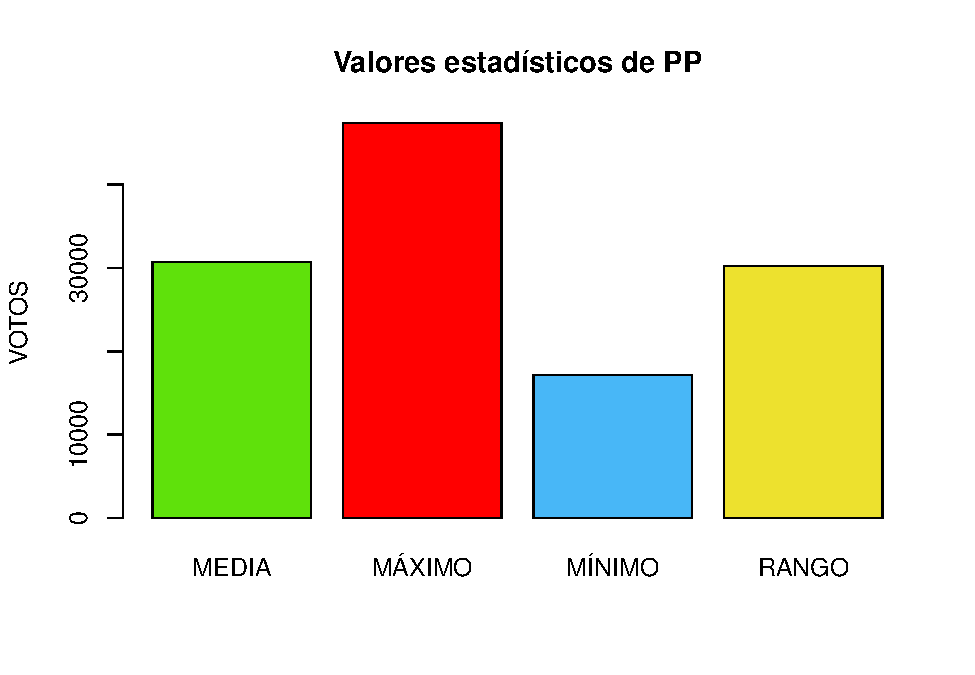
\includegraphics{SAFOR_files/figure-latex/6-1.pdf}

\begin{longtable}[]{@{}lr@{}}
\caption{ESTADÍSTICA SAFOR PP}\tabularnewline
\toprule\noalign{}
ESTADÍSTICA & VALORS \\
\midrule\noalign{}
\endfirsthead
\toprule\noalign{}
ESTADÍSTICA & VALORS \\
\midrule\noalign{}
\endhead
\bottomrule\noalign{}
\endlastfoot
MEDIA & 30729 \\
MÁXIMO & 47413 \\
MÍNIMO & 17142 \\
RANGO & 30271 \\
\end{longtable}

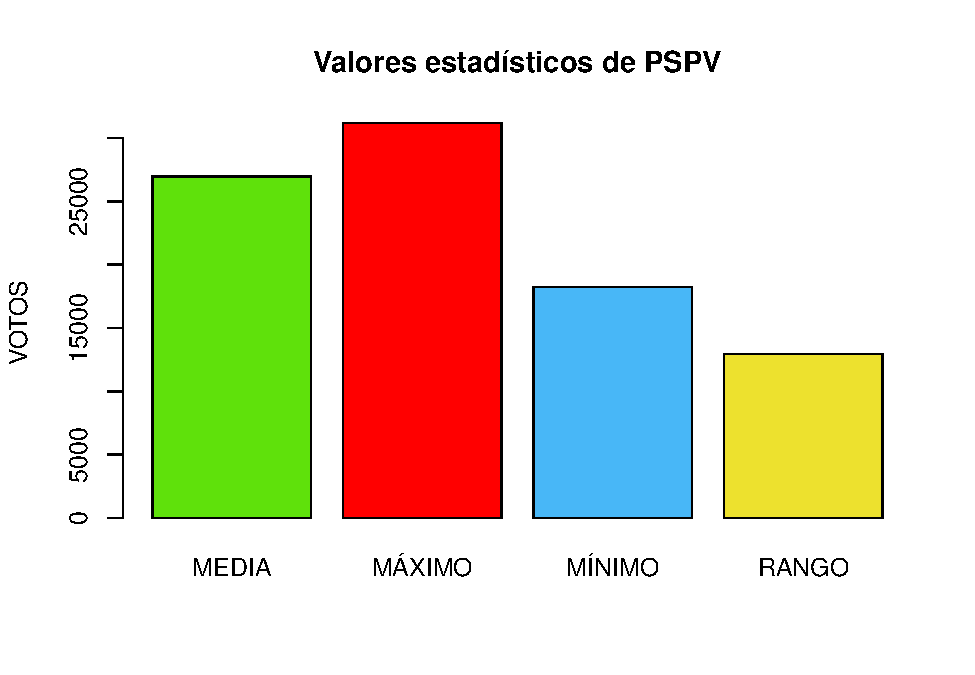
\includegraphics{SAFOR_files/figure-latex/6-2.pdf}

\begin{longtable}[]{@{}lr@{}}
\caption{ESTADÍSTICA SAFOR PSPV}\tabularnewline
\toprule\noalign{}
ESTADÍSTICA & VALORS \\
\midrule\noalign{}
\endfirsthead
\toprule\noalign{}
ESTADÍSTICA & VALORS \\
\midrule\noalign{}
\endhead
\bottomrule\noalign{}
\endlastfoot
MEDIA & 26985 \\
MÁXIMO & 31192 \\
MÍNIMO & 18226 \\
RANGO & 12966 \\
\end{longtable}

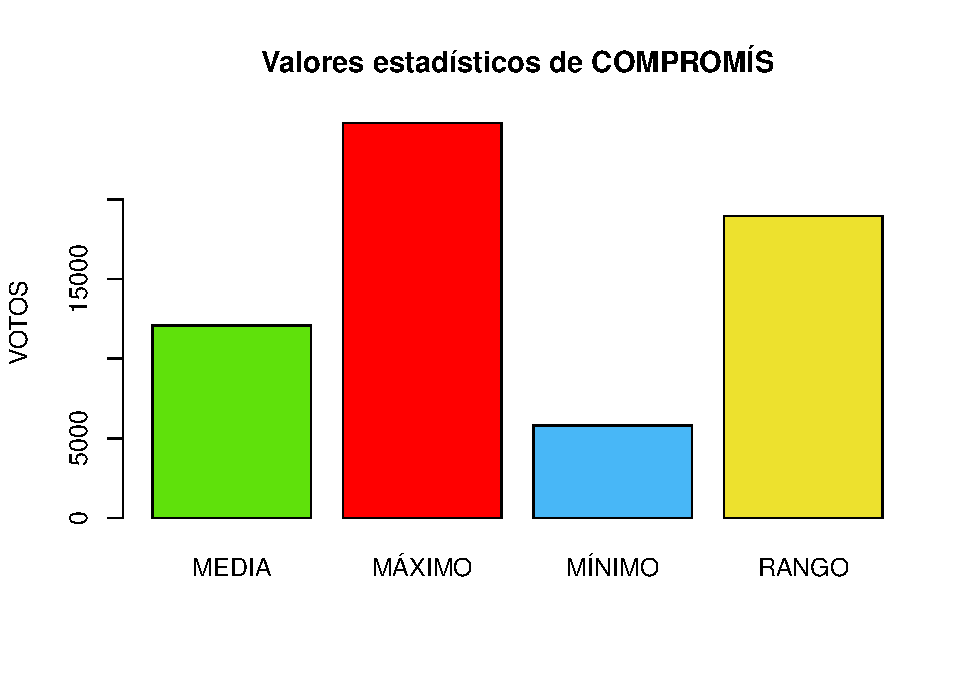
\includegraphics{SAFOR_files/figure-latex/6-3.pdf}

\begin{longtable}[]{@{}lr@{}}
\caption{ESTADÍSTICA SAFOR COMPROMÍS}\tabularnewline
\toprule\noalign{}
ESTADÍSTICA & VALORS \\
\midrule\noalign{}
\endfirsthead
\toprule\noalign{}
ESTADÍSTICA & VALORS \\
\midrule\noalign{}
\endhead
\bottomrule\noalign{}
\endlastfoot
MEDIA & 12094 \\
MÁXIMO & 24789 \\
MÍNIMO & 5823 \\
RANGO & 18966 \\
\end{longtable}

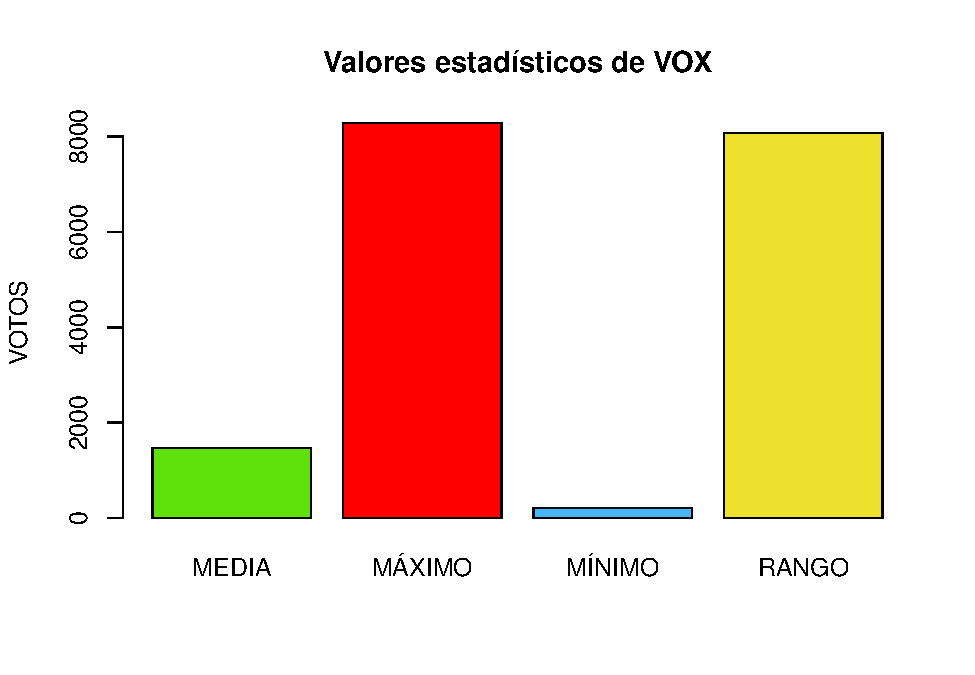
\includegraphics{SAFOR_files/figure-latex/6-4.pdf}

\begin{longtable}[]{@{}lr@{}}
\caption{ESTADÍSTICA SAFOR VOX}\tabularnewline
\toprule\noalign{}
ESTADÍSTICA & VALORS \\
\midrule\noalign{}
\endfirsthead
\toprule\noalign{}
ESTADÍSTICA & VALORS \\
\midrule\noalign{}
\endhead
\bottomrule\noalign{}
\endlastfoot
MEDIA & 1468 \\
MÁXIMO & 8282 \\
MÍNIMO & 207 \\
RANGO & 8075 \\
\end{longtable}

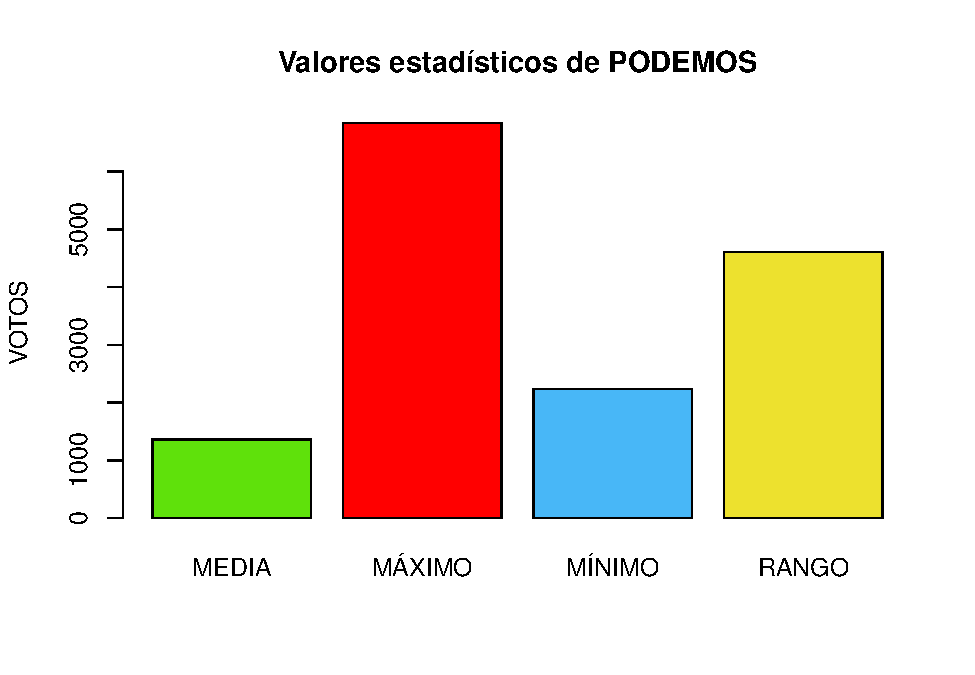
\includegraphics{SAFOR_files/figure-latex/6-5.pdf}

\begin{longtable}[]{@{}lr@{}}
\caption{ESTADÍSTICA SAFOR PODEMOS}\tabularnewline
\toprule\noalign{}
ESTADÍSTICA & VALORS \\
\midrule\noalign{}
\endfirsthead
\toprule\noalign{}
ESTADÍSTICA & VALORS \\
\midrule\noalign{}
\endhead
\bottomrule\noalign{}
\endlastfoot
MEDIA & 1363 \\
MÁXIMO & 6845 \\
MÍNIMO & 2234 \\
RANGO & 4611 \\
\end{longtable}

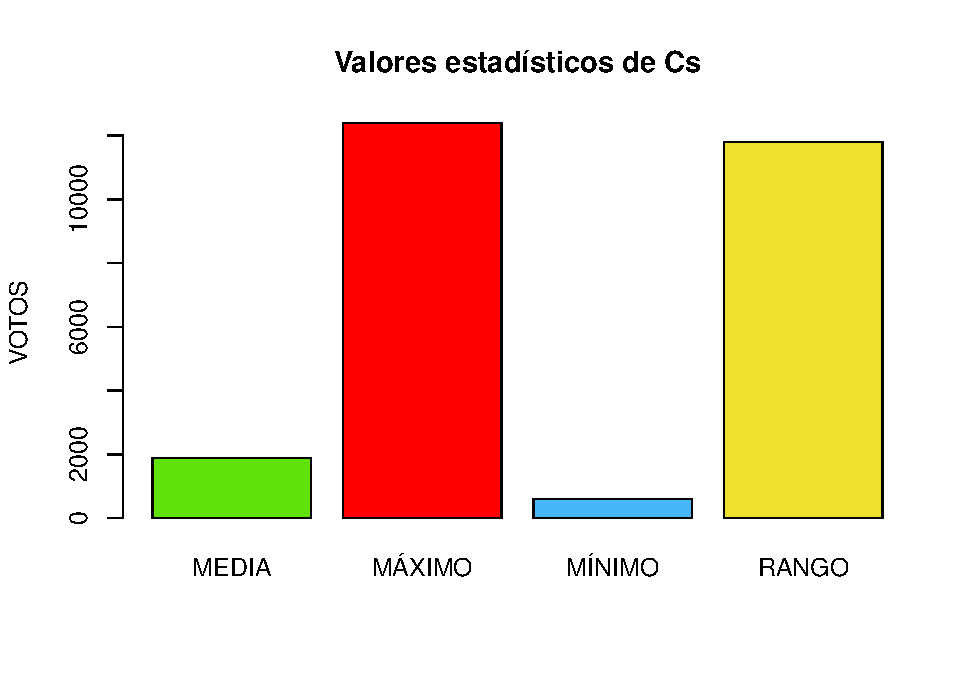
\includegraphics{SAFOR_files/figure-latex/6-6.pdf}

\begin{longtable}[]{@{}lr@{}}
\caption{ESTADÍSTICA SAFOR Cs}\tabularnewline
\toprule\noalign{}
ESTADÍSTICA & VALORS \\
\midrule\noalign{}
\endfirsthead
\toprule\noalign{}
ESTADÍSTICA & VALORS \\
\midrule\noalign{}
\endhead
\bottomrule\noalign{}
\endlastfoot
MEDIA & 1877 \\
MÁXIMO & 12394 \\
MÍNIMO & 591 \\
RANGO & 11803 \\
\end{longtable}

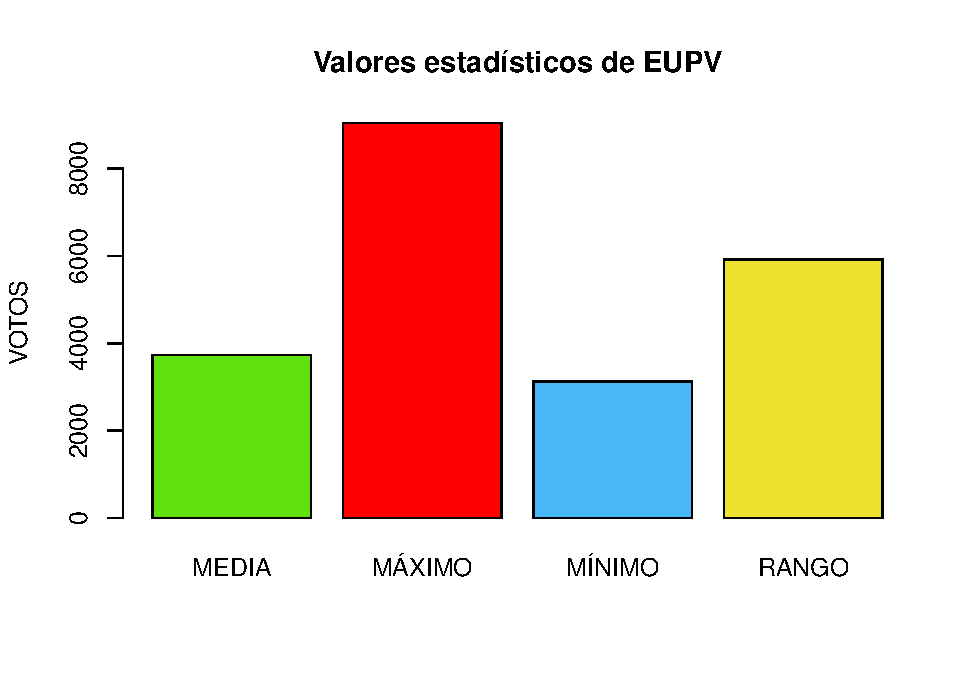
\includegraphics{SAFOR_files/figure-latex/6-7.pdf}

\begin{longtable}[]{@{}lr@{}}
\caption{ESTADÍSTICA SAFOR EUPV}\tabularnewline
\toprule\noalign{}
ESTADÍSTICA & VALORS \\
\midrule\noalign{}
\endfirsthead
\toprule\noalign{}
ESTADÍSTICA & VALORS \\
\midrule\noalign{}
\endhead
\bottomrule\noalign{}
\endlastfoot
MEDIA & 3732 \\
MÁXIMO & 9042 \\
MÍNIMO & 3129 \\
RANGO & 5913 \\
\end{longtable}

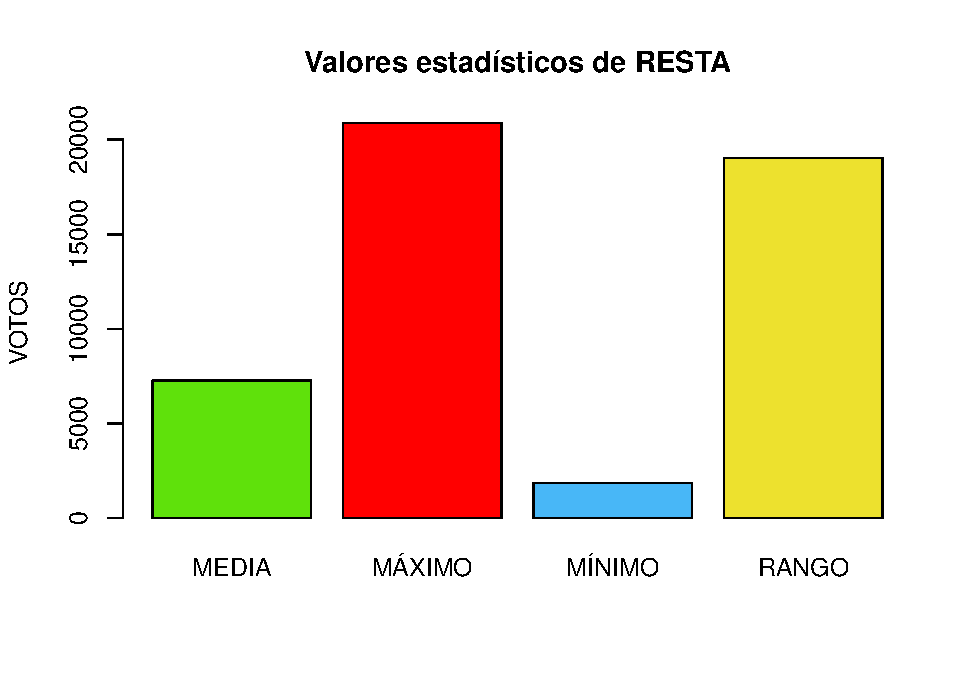
\includegraphics{SAFOR_files/figure-latex/6-8.pdf}

\begin{longtable}[]{@{}lr@{}}
\caption{ESTADÍSTICA SAFOR RESTA}\tabularnewline
\toprule\noalign{}
ESTADÍSTICA & VALORS \\
\midrule\noalign{}
\endfirsthead
\toprule\noalign{}
ESTADÍSTICA & VALORS \\
\midrule\noalign{}
\endhead
\bottomrule\noalign{}
\endlastfoot
MEDIA & 7255 \\
MÁXIMO & 20879 \\
MÍNIMO & 1859 \\
RANGO & 19020 \\
\end{longtable}

\hypertarget{guardar-data-frame-en-ficheros-de-diferentes-formatos}{%
\section{GUARDAR DATA FRAME EN FICHEROS DE DIFERENTES
FORMATOS}\label{guardar-data-frame-en-ficheros-de-diferentes-formatos}}

\hypertarget{guardar-datos-en-formato-.xlsx-ms-excel}{%
\subsection{Guardar datos en formato .xlsx (MS
Excel)}\label{guardar-datos-en-formato-.xlsx-ms-excel}}

Se instala el paquete solo si hace falta

\begin{Shaded}
\begin{Highlighting}[]
\ControlFlowTok{if}\NormalTok{ (}\SpecialCharTok{!}\FunctionTok{require}\NormalTok{(}\StringTok{"xlsx"}\NormalTok{)) \{}\FunctionTok{install.packages}\NormalTok{(}\StringTok{"xlsx"}\NormalTok{)\}}
\end{Highlighting}
\end{Shaded}

\begin{verbatim}
## Loading required package: xlsx
\end{verbatim}

Se creará un fichero de tipo MS Excel: \emph{resultats.xlsx}

\begin{Shaded}
\begin{Highlighting}[]
\DocumentationTok{\#\#\# Creando un nuevo fichero xlsx}

\FunctionTok{write.xlsx}\NormalTok{(df\_resultats, }\AttributeTok{file =} \StringTok{"resultats.xlsx"}\NormalTok{, }\AttributeTok{sheetName =} \StringTok{"resultats"}\NormalTok{, }\AttributeTok{append =} \ConstantTok{FALSE}\NormalTok{)}
\end{Highlighting}
\end{Shaded}

\hypertarget{auxf1adiendo-una-hoja-en-un-ficher-xlsx-existente}{%
\subsection{Añadiendo una hoja en un ficher xlsx
existente}\label{auxf1adiendo-una-hoja-en-un-ficher-xlsx-existente}}

Aquí añadiremos una página más a un fichero MS Excel existente
(append=TRUE). Si \emph{ficheroAnterior.xlsx} no existe dará error.

\begin{Shaded}
\begin{Highlighting}[]
\FunctionTok{write.xlsx}\NormalTok{(df\_resultats, }\AttributeTok{file =} \StringTok{"ficheroAnterior.xlsx"}\NormalTok{, }\AttributeTok{sheetName=}\StringTok{"resultats"}\NormalTok{, }\AttributeTok{append=}\ConstantTok{TRUE}\NormalTok{)}
\end{Highlighting}
\end{Shaded}

\hypertarget{guardar-datos-en-formato-.dta-stata.}{%
\subsection{Guardar datos en formato .dta /
Stata.}\label{guardar-datos-en-formato-.dta-stata.}}

\begin{Shaded}
\begin{Highlighting}[]
\ControlFlowTok{if}\NormalTok{ (}\SpecialCharTok{!}\FunctionTok{require}\NormalTok{(}\StringTok{"foreign"}\NormalTok{)) \{}\FunctionTok{install.packages}\NormalTok{(}\StringTok{"foreign"}\NormalTok{)\}}
\FunctionTok{write.dta}\NormalTok{(df\_resultats, }\StringTok{"resultats.dta"}\NormalTok{)}
\end{Highlighting}
\end{Shaded}

\hypertarget{guardar-datos-en-formato-.csv}{%
\subsection{Guardar datos en formato
.csv}\label{guardar-datos-en-formato-.csv}}

\begin{Shaded}
\begin{Highlighting}[]
\ControlFlowTok{if}\NormalTok{ (}\SpecialCharTok{!}\FunctionTok{require}\NormalTok{(}\StringTok{"tidyverse"}\NormalTok{)) \{}\FunctionTok{install.packages}\NormalTok{(}\StringTok{"tidyverse"}\NormalTok{)\}}
\FunctionTok{write\_csv}\NormalTok{(df\_resultats, }\StringTok{"resultats.csv"}\NormalTok{)}
\end{Highlighting}
\end{Shaded}

\hypertarget{guardar-datos-en-formato-.sav-spss}{%
\subsection{Guardar datos en formato .sav /
SPSS}\label{guardar-datos-en-formato-.sav-spss}}

\begin{Shaded}
\begin{Highlighting}[]
\ControlFlowTok{if}\NormalTok{ (}\SpecialCharTok{!}\FunctionTok{require}\NormalTok{(}\StringTok{"haven"}\NormalTok{)) \{}\FunctionTok{install.packages}\NormalTok{(}\StringTok{"haven"}\NormalTok{)\}}
\FunctionTok{write\_sav}\NormalTok{(df\_resultats, }\StringTok{"resultats.sav"}\NormalTok{)}
\end{Highlighting}
\end{Shaded}

\hypertarget{guardar-y-abrir-datos-en-formato-rstudio.}{%
\subsection{Guardar y abrir datos en formato
RStudio.}\label{guardar-y-abrir-datos-en-formato-rstudio.}}

No es lo más usado, porque la costumbre es compartir los datos en
formatos como .csv u otros que sean más comunes. No obstante, conviene
conocer estos formatos, que se manejan muy fácilmente. No requieren
librería, pues estos comandos trabajan con las funciones que trae
\textbf{RStudio}.

\begin{quote}
RData - permite guardar más de una base de datos en un mismo archivo.
\end{quote}

\begin{Shaded}
\begin{Highlighting}[]
\FunctionTok{save}\NormalTok{(df\_resultats, }\AttributeTok{file=}\StringTok{"resultats.RData"}\NormalTok{)}
\end{Highlighting}
\end{Shaded}

\hypertarget{lectura-de-datos-rdata}{%
\subsection{Lectura de datos RData}\label{lectura-de-datos-rdata}}

El parámetro \emph{verbose=TRUE} es opcional. Sirve para que en la carga
(lectura) nos muestre los datos (dataframe en este caso) existentes en
el fichero de tipo \emph{.Rdata}. en nuestro ejemplo vemos que contiene
el dataframe: \emph{df\_resultats}

\begin{Shaded}
\begin{Highlighting}[]
\FunctionTok{load}\NormalTok{(}\StringTok{"resultats.RData"}\NormalTok{,}\AttributeTok{verbose=}\ConstantTok{TRUE}\NormalTok{)}
\end{Highlighting}
\end{Shaded}

\begin{verbatim}
## Loading objects:
##   df_resultats
\end{verbatim}

\hypertarget{rds---guarda-un-solo-archivo-de-datos}{%
\subsection{RDS - guarda un solo archivo de
datos}\label{rds---guarda-un-solo-archivo-de-datos}}

\begin{Shaded}
\begin{Highlighting}[]
\FunctionTok{saveRDS}\NormalTok{(df\_resultats, }\StringTok{"resultats.rds"}\NormalTok{)}
\end{Highlighting}
\end{Shaded}

\hypertarget{lectura-de-datos-rds}{%
\subsection{Lectura de datos RDS}\label{lectura-de-datos-rds}}

\begin{Shaded}
\begin{Highlighting}[]
\NormalTok{df\_resultats2 }\OtherTok{\textless{}{-}} \FunctionTok{readRDS}\NormalTok{(}\StringTok{"resultats.rds"}\NormalTok{)}
\end{Highlighting}
\end{Shaded}


\end{document}
